\documentclass[nobib]{tufte-handout}
\usepackage{amsmath,amssymb,amsthm}
\usepackage[pdftex]{graphicx}

\title{COMP 210 \\ Lecture Notes 02 \\ Java Program Structure and Eclipse}

\begin{document}
\maketitle

\begin{abstract}
In these notes we talk about the basic structure of Java-based OOP programs and how to setup and build them with the Eclipse IDE\@. We'll more or less ignore Java syntax for now as the code that's written in this process is written by the IDE\@.
\end{abstract}

\section{Overview}

All code in Java \textit{must} be in a class or something similar\sidenote{You'll learn about some other class-like definitions}. \textit{A source file can only contain one public class and the file name must match the class name}. So, if programs are built from the interaction of many objects and we need multiple classes to define the types of those objects, then we're quickly going to be dealing with programs whose code is spread across many, many files. Classes are organized within \textit{packages}. Just like we did with C++ namespaces, we'll always define our classes within packages. Not using packages is not good style. Package placement will also have an impact on the scope of the definition as well.

We'll continue to use unit testing in the design and implementation of our programs.  The go-to framework in Java is JUnit\sidenote{\url{http://junit.org}}. You'll find it's very similar to GTest. Just like before we'll separate tests from code. Each class will get its own file of tests, which will also be a class of course. That class will typically get placed in the same package as the class its testing.

To start out we'll work with programs composed of several classes that are defined in separate files and done so relative to a package.


\section{Eclipse Projects and Project Structure}

Eclipse is a programming IDE\@. It's written and Java and very well suited for Java development. Through plug-ins you can use it for a wide variety of other languages as well. As a batteries included IDE it includes a robust text editor, integrates with a compiler, and allows you to run and debug programs from within the IDE itself.

Programs in Eclipse are represented as \textit{projects}. Projects are organized within a \textit{workspace}. The workspace corresponds to directory and the program to a sub-directory of the workspace directory. When you start Eclipse you'll be prompted to select a workspace.

\vspace{.1in}
\begin{center}
\begin{figure}
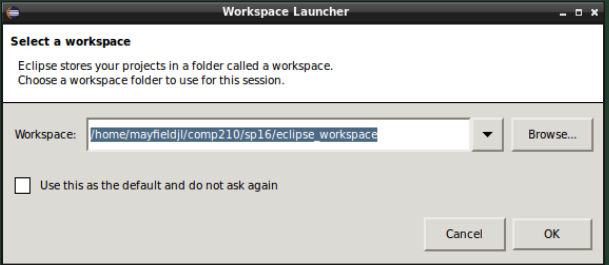
\includegraphics[scale=.5]{Eclipse-select-workspace.png}
\caption{The Eclipse workspace selection window}
\end{figure}
\end{center}
\vspace{.1in}


I recommend you create a class specific workspace, either way, make a fresh, new directory to act as your Eclipse workspace. You can also check the box to make this the default. You can always switch workspace from the File menu in Eclipse.

The first time you launch Eclipse you're greeted with a Welcome screen. Just click the icon to take you to the workbench, where we'll be working.

\vspace{.1in}
\begin{center}
\begin{figure}
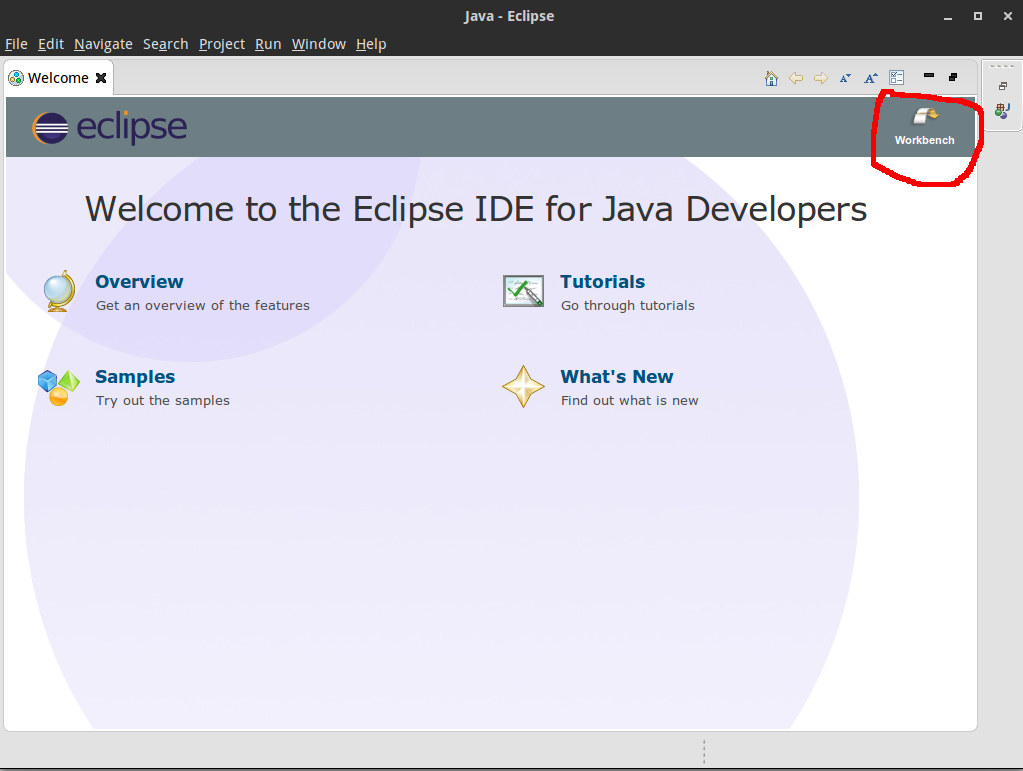
\includegraphics[scale=.25]{Eclipse-Welcome.png}
\caption{The Eclipse Welcome Screen. Just go to the Workbench.}
\end{figure}
\end{center}
\vspace{.1in}

You're now ready to create a \textit{Java Project} you can do this in the usual ways, from File > New or the New Quick button. Once there, choose a project name and ensure your settings look like those in figure~\ref{fig:newproj}. Then click Next.

\vspace{.1in}
\begin{center}
\begin{figure}[!htb]
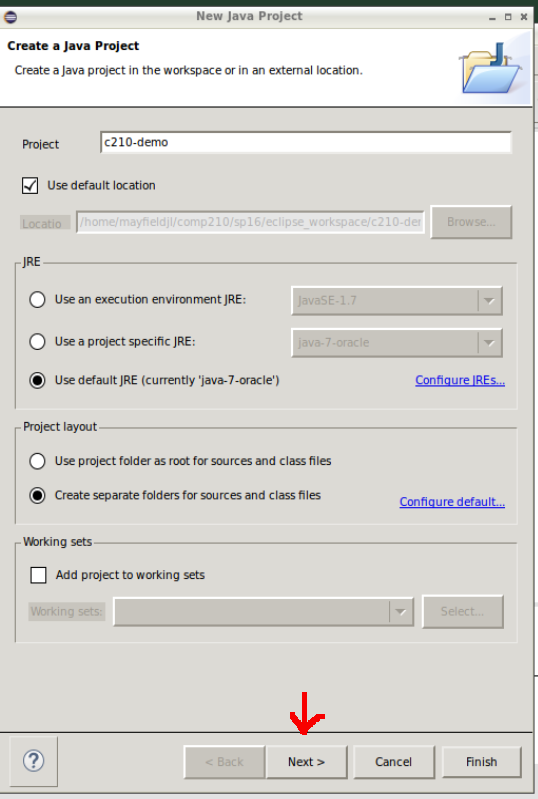
\includegraphics[scale=.3]{Eclipse-NewProject.png}
\caption{First Screen in New Project Dialog}
\label{fig:newproj}
\end{figure}
\end{center}
\vspace{.1in}

Next we need to do some setup for using our unit-testing framework JUnit4\sidenote{\url{http://junit.org/}}. There are two things to do: create a folder to hold all out test code and add the JUnit library to the project. The folder is optional, but we'll be keeping tests separated from our actual code. To create the folder you'll hit the new source folder link. In the dialog that pops up, name the new folder \textit{tests} and click Finish. You can see this in figure~\ref{fig:newsrcfold}

\vspace{.1in}
\begin{center}
\begin{figure}[!htb]
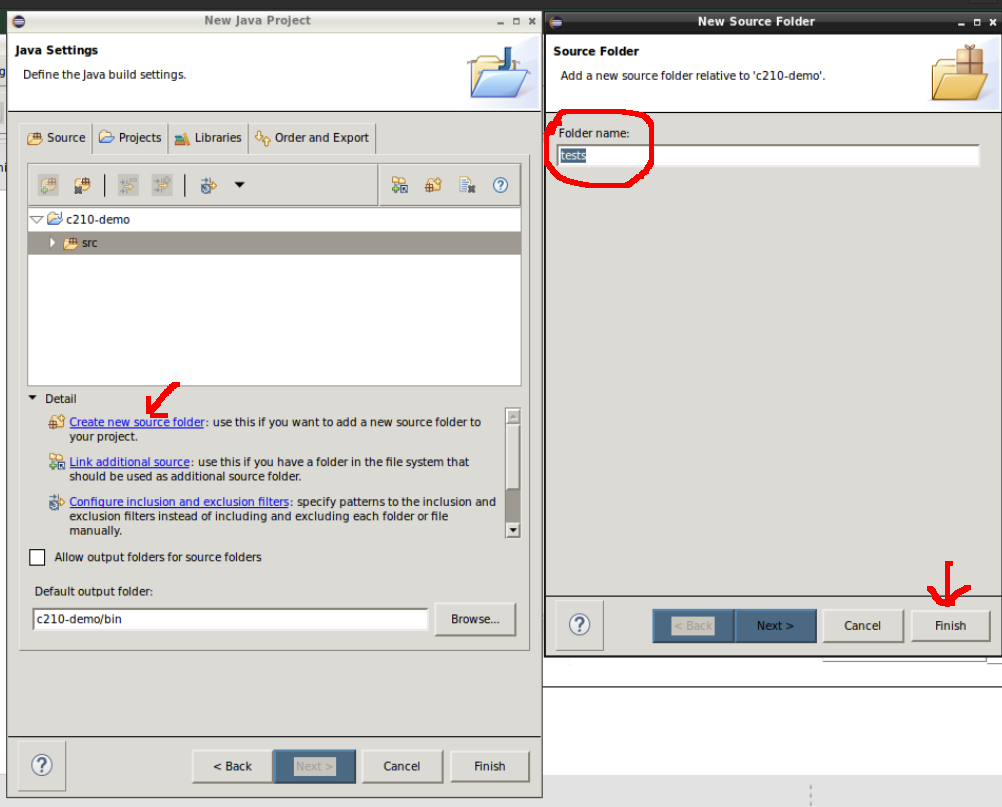
\includegraphics[scale=.3]{Eclipse-AddTestFolder.png}
\caption{First Screen in New Project Dialog}
\label{fig:newsrcfold}
\end{figure}
\end{center}
\vspace{.1in}

To add the JUnit library itself, you need to select the \textit{Libraries} tab then select JUnit in the dialog that pops up. Then press the Next button. You can see this in figure~\ref{fig:AddJUnitLib}. The last window ensures you have the right version of JUnit. It should look like figure~\ref{fig:SelectJUnit4}.

\vspace{.1in}
\begin{center}
\begin{figure}[!htb]
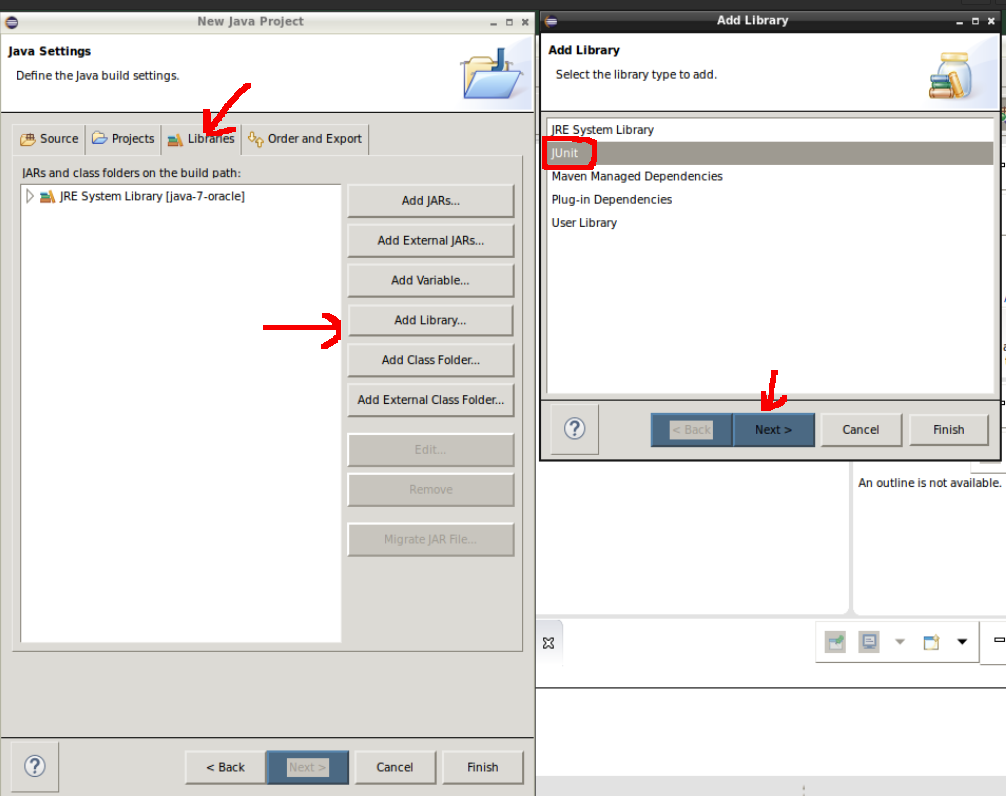
\includegraphics[scale=.3]{Eclipse-AddJUnitLib.png}
\caption{Dialogs for Adding JUnit to a Project}
\label{fig:AddJUnitLib}
\end{figure}
\end{center}
\vspace{.1in}


\vspace{.1in}
\begin{center}
\begin{figure}[!htb]
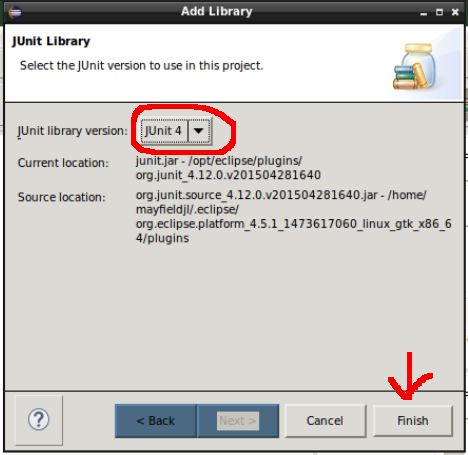
\includegraphics[scale=.5]{Eclipse-SelectJUnit4.png}
\caption{Dialog to Select version 4 of JUnit }
\label{fig:SelectJUnit4}
\end{figure}
\end{center}
\vspace{.1in}

Once you've setup the test folder and library, you're project is all setup.

\subsection{Packages}

Before we start creating classes we need to create a package or two for those classes. Packages are created within source folders and correspond to physical sub-directories within that folder. So, unlike C++ Namespaces, packages have a physical presence.

If our tests and classes are going in the same package then we need to create that package twice, once in the \textit{src} folder and once in the test folder. There are at least three ways to create a new package: File > New, the New quick button, and right clicking the folder in which the package is to be placed. In either case you end up at a dialog like figure~\ref{fig:newpackage} that lets you specify the parent director and name of the new package. \textbf{The name of your package should start with a lower case letter}\sidenote{Eclipse will warn you if you use Uppercase}. This is a convention and not a syntax error.  You should consider it an error though as you'll lose points for violating the convention.

\vspace{.1in}
\begin{center}
\begin{figure}[h]
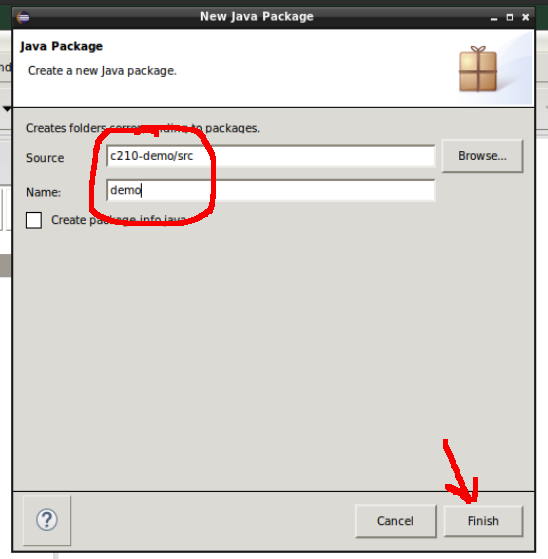
\includegraphics[scale=.5]{Eclipse-NewPackage.png}
\caption{New Package Dialog}
\label{fig:newpackage}
\end{figure}
\end{center}
\vspace{.1in}


When you're done your project should show the packages within their respective source folders as seen in figure~\ref{fig:projWithPacks}.

\vspace{.1in}
\begin{center}
\begin{figure}[h]
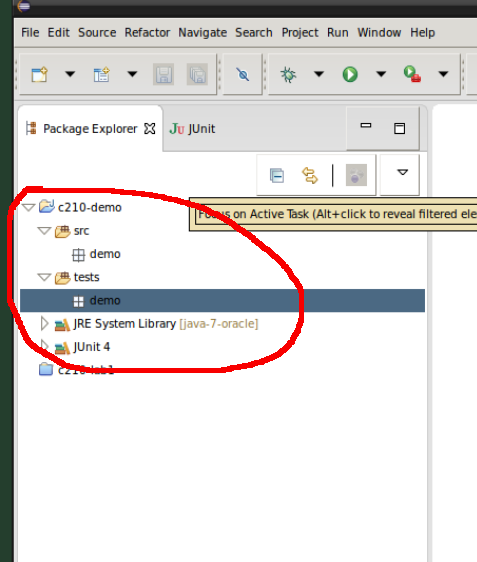
\includegraphics[scale=.5]{Eclipse-ProjectWithPacks.png}
\caption{A Project with src and tests folders and a shared package}
\label{fig:projWithPacks}
\end{figure}
\end{center}
\vspace{.1in}

With packages in place, we're ready to start creating Classes, i.e.\ source files.

\section{Classes and Files}

To create a new Class you an use the usual options: File $>$ New, the New quick button, or right click New on the package in which you want the Class placed. We'll always start by stubbing out the class. We can then use Eclipse to stub out the tests. You'll find that Eclipse can auto-generate a lot of boiler place code for you. This is good because it'll save time. It's bad because it's all too easy for you to ignore that code and not know how to write it yourself. This will undoubtedly lead to you losing points on quizzes and exams or botching an interview for an internship or job. So, \textit{just because the IDE writes the code for you doesn't mean you don't need to know how to do it yourself!}

The new Class dialog has lots of options. We'll deal with them on an as needed basis. The core options are specifying the location, package, and name of the class. \textbf{The class name should start with an uppercase letter}. This is, again, a convention that we'll follow as a rule. The class name becomes the file name. Java files have the unsurprising extension of \textit{java}. Figure~\ref{fig:newclass} points the core options and one extra option, stubbing out a \textit{main}, that's discussed a bit below.

\vspace{.1in}
\begin{center}
\begin{figure}[h]
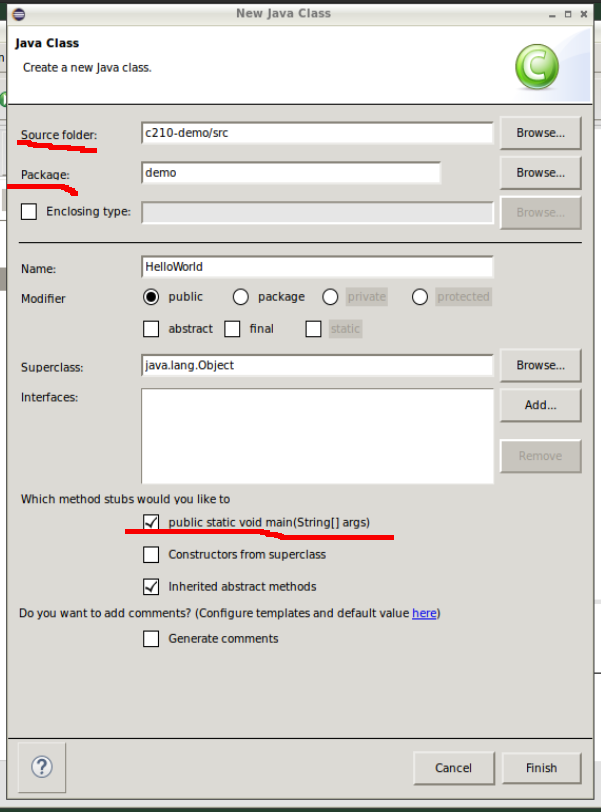
\includegraphics[scale=.5]{Eclipse-NewClass.png}
\caption{New Class Dialog with core options highlighted.}
\label{fig:newclass}
\end{figure}
\end{center}
\vspace{.1in}

\subsection{The \textit{main} procedure}

The other New Class dialog option I'll point out now is that this dialog give you the option to automatically generate a stub for \textit{main}.  Java, like C++, operates by executing a \textit{main} procedure. It's the one procedure we'll write with any kind of regularity.

\section{Compile and Run}

In figure~\ref{fig:helloworld} you'll see a Hello World program in Java. We'll leave the details of the code itself for the next set of notes. For now you should notice a few things highlighted in the figure. The green play button compiles and runs the program. Console output\sidenote{and input} happens down at the bottom. In code, the inclusion of a file/class in a package takes place with a simple package declaration. Files are opened and edited in the center of the window. IF you've been following along, then you're encouraged to play around a bit. Go find some other Java tutorials and make a more interesting Hello World. In the next set of notes we'll design, document, implement, and test some procedures in order to get a better feel for the nuts and bolts of Java.


\vspace{.1in}
\begin{center}
\begin{figure}[h]
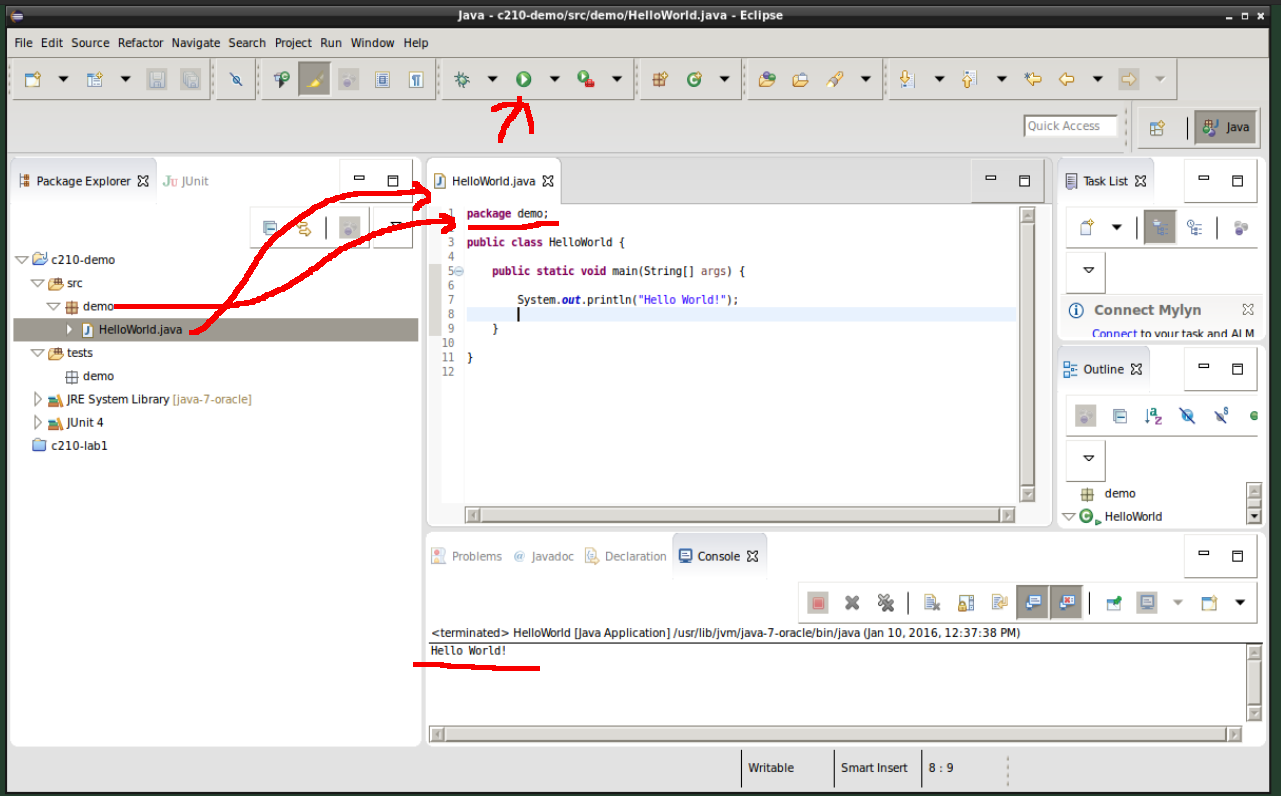
\includegraphics[scale=.25]{Eclipse-HelloWorld.png}
\caption{Hello World in Java}
\label{fig:helloworld}
\end{figure}
\end{center}
\vspace{.1in}

\end{document}
